\documentclass{beamer}
\usepackage{ragged2e}
\usepackage{CJKutf8}
\usepackage{tikz}
\setbeamertemplate{theorems}[numbered]
\newtheorem{Exercise}{习题}

\begin{document}
\begin{CJK*}{UTF8}{gbsn}

  \newtheorem{Thm}{定理}[section]
  \newtheorem*{Thm1}{定理1.1}
  \newtheorem*{Thm2}{定理}
\theoremstyle{definition}
\newtheorem{Def}{定义}[section]
\theoremstyle{example}
\newtheorem*{Ex}{例:}
\date{}
\author{陈建文}

\title{第七章 树和割集}
\begin{frame}
  \titlepage
\end{frame}  
\section{树及其性质}
\begin{frame}
  \frametitle{1. 树及其性质}
      \begin{minipage}{0.49\linewidth}
    \centering
    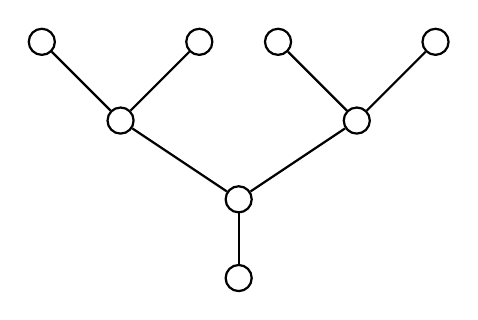
\begin{tikzpicture}[auto,
    specification/.style ={circle, draw, thick}]
   \node[specification] (A)  at (0,0)  {};
   \node[specification] (B)  at (0,1)  {};
   \node[specification] (C)  at (-1.5,2)  {};
   \node[specification] (D)  at (-2.5,3)  {};
   \node[specification] (E)  at (-0.5,3)  {};
   \node[specification] (F)  at (1.5,2)  {};
   \node[specification] (G)  at (0.5,3)  {};
   \node[specification] (H)  at (2.5,3)  {};

   \draw[thick] (A) to  (B);
   \draw[thick] (B) to (C);
   \draw[thick] (C) to (D);
   \draw[thick] (C) to (E);
   \draw[thick] (B) to (F);
   \draw[thick] (F) to (G);
   \draw[thick] (F) to (H);
 \end{tikzpicture}
\end{minipage}\pause
    \begin{minipage}{0.49\linewidth}
    \centering
    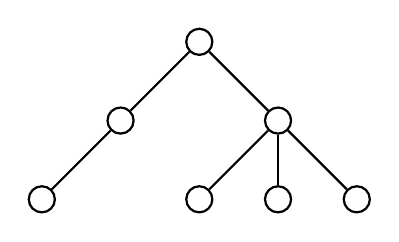
\begin{tikzpicture}[auto,
    specification/.style ={circle, draw, thick}]
   \node[specification] (A)  at (0,0)  {};
   \node[specification] (B)  at (-1,-1)  {};
   \node[specification] (C)  at (1,-1)  {};
   \node[specification] (D)  at (-2,-2)  {};
   \node[specification] (E)  at (0,-2)  {};
   \node[specification] (F)  at (1,-2)  {};
   \node[specification] (G)  at (2,-2)  {};

   \draw[thick] (A) to  (B);
   \draw[thick] (A) to (C);
   \draw[thick] (B) to (D);
   \draw[thick] (C) to (E);
   \draw[thick] (C) to (F);
   \draw[thick] (C) to (G);   
 \end{tikzpicture}
\end{minipage}
\end{frame}

\begin{frame}
  \frametitle{1. 树及其性质}
  \begin{Def}
    连通且无圈的无向图称为无向树,简称\alert{树}。
  \end{Def}
\pause \centering
  \begin{minipage}{0.24\linewidth}
    \centering
    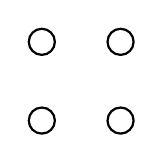
\begin{tikzpicture}[auto,
    specification/.style ={circle, draw, thick}]
   \node[specification] (A) at (0,0)  {};
   \node[specification] (B)  at (0,1)  {};
   \node[specification] (C)  at (1,1)  {};
   \node[specification] (D) at (1,0)  {};
 \end{tikzpicture}\\
 \vspace*{0.1cm}
 A
\end{minipage}\hfill 
  \begin{minipage}{0.24\linewidth}
    \centering
    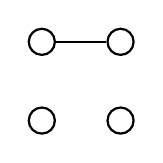
\begin{tikzpicture}[auto,
    specification/.style ={circle, draw, thick}]
   \node[specification] (A) at (0,0)  {};
   \node[specification] (B) at (0,1)  {};
   \node[specification] (C) at (1,1)  {};
   \node[specification] (D) at (1,0)  {};
   \draw[thick] (B) to  (C);
 \end{tikzpicture}\\
 \vspace*{0.1cm}
 B
\end{minipage}\hfill 
  \begin{minipage}{0.24\linewidth}
    \centering
    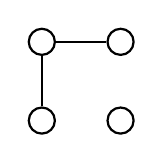
\begin{tikzpicture}[auto,
    specification/.style ={circle, draw, thick}]
   \node[specification] (A) at (0,0)  {};
   \node[specification] (B) at (0,1)  {};
   \node[specification] (C) at (1,1)  {};
   \node[specification] (D) at (1,0)  {};
   \draw[thick] (A) to  (B);
   \draw[thick] (B) to  (C);
 \end{tikzpicture}\\
 \vspace*{0.1cm}
 C
\end{minipage}\hfill 
  \begin{minipage}{0.24\linewidth}
    \centering
    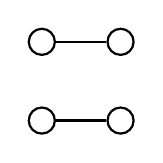
\begin{tikzpicture}[auto,
    specification/.style ={circle, draw, thick}]
   \node[specification] (A)  at (0,0)  {};
   \node[specification] (B)  at (0,1)  {};
   \node[specification] (C)  at (1,1)  {};
   \node[specification] (D) at (1,0)  {};
   \draw[thick] (B) to  (C);
   \draw[thick] (D) to  (A);
 \end{tikzpicture}\\
 \vspace*{0.1cm}
 D
\end{minipage}\hfill

\vspace*{0.5cm}
  \begin{minipage}{0.24\linewidth}
    \centering
    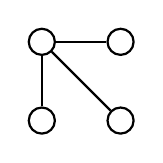
\begin{tikzpicture}[auto,
    specification/.style ={circle, draw, thick}]
   \node[specification] (A) at (0,0)  {};
   \node[specification] (B)  at (0,1)  {};
   \node[specification] (C)  at (1,1)  {};
   \node[specification] (D) at (1,0)  {};
   \draw[thick] (A) to (B);
   \draw[thick] (B) to (C);
      \draw[thick] (B) to (D);
 \end{tikzpicture}\\
 \vspace*{0.1cm}
 E
\end{minipage}\hfill
  \begin{minipage}{0.24\linewidth}
    \centering
    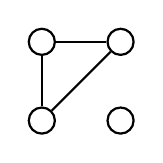
\begin{tikzpicture}[auto,
    specification/.style ={circle, draw, thick}]
   \node[specification] (A) at (0,0)  {};
   \node[specification] (B) at (0,1)  {};
   \node[specification] (C) at (1,1)  {};
   \node[specification] (D) at (1,0)  {};
   \draw[thick] (A) to  (B);
   \draw[thick] (B) to (C);
   \draw[thick] (C) to (A);
 \end{tikzpicture}\\
 \vspace*{0.1cm}
 F
\end{minipage}\hfill
  \begin{minipage}{0.24\linewidth}
    \centering
    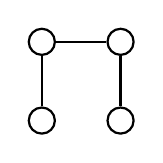
\begin{tikzpicture}[auto,
    specification/.style ={circle, draw, thick}]
   \node[specification] (A) at (0,0)  {};
   \node[specification] (B) at (0,1)  {};
   \node[specification] (C) at (1,1)  {};
   \node[specification] (D) at (1,0)  {};
   \draw[thick] (A) to  (B);
   \draw[thick] (B) to  (C);
      \draw[thick] (C) to (D);
 \end{tikzpicture}\\
 \vspace*{0.1cm}
 G
\end{minipage}\hfill 
  \begin{minipage}{0.24\linewidth}
    \centering
    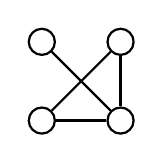
\begin{tikzpicture}[auto,
    specification/.style ={circle, draw, thick}]
   \node[specification] (A)  at (0,0)  {};
   \node[specification] (B)  at (0,1)  {};
   \node[specification] (C)  at (1,1)  {};
   \node[specification] (D) at (1,0)  {};
   \draw[thick] (A) to  (C);
   \draw[thick] (C) to  (D);
   \draw[thick] (D) to (A);
   \draw[thick] (B) to (D);
 \end{tikzpicture}\\
 \vspace*{0.1cm}
 H
\end{minipage}\hfill 

\vspace*{0.5cm}
\flushleft
  \begin{minipage}{0.24\linewidth}
    \centering
    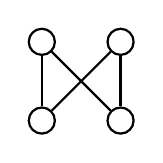
\begin{tikzpicture}[auto,
    specification/.style ={circle, draw, thick}]
   \node[specification] (A) at (0,0)  {};
   \node[specification] (B)  at (0,1)  {};
   \node[specification] (C)  at (1,1)  {};
   \node[specification] (D) at (1,0)  {};
   \draw[thick] (A) to (B);
   \draw[thick] (B) to (D);
   \draw[thick] (D) to (C);
      \draw[thick] (C) to (A);
 \end{tikzpicture}\\
 \vspace*{0.1cm}
 I
\end{minipage}
  \begin{minipage}{0.24\linewidth}
    \centering
    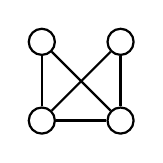
\begin{tikzpicture}[auto,
    specification/.style ={circle, draw, thick}]
   \node[specification] (A) at (0,0)  {};
   \node[specification] (B) at (0,1)  {};
   \node[specification] (C) at (1,1)  {};
   \node[specification] (D) at (1,0)  {};
   \draw[thick] (A) to  (B);
      \draw[thick] (C) to (D);
   \draw[thick] (D) to (A);
   \draw[thick] (A) to (C);
   \draw[thick] (B) to (D);
 \end{tikzpicture}\\
 \vspace*{0.1cm}
 J
\end{minipage} 
  \begin{minipage}{0.24\linewidth}
    \centering
    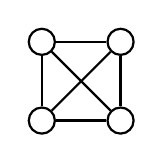
\begin{tikzpicture}[auto,
    specification/.style ={circle, draw, thick}]
   \node[specification] (A) at (0,0)  {};
   \node[specification] (B) at (0,1)  {};
   \node[specification] (C) at (1,1)  {};
   \node[specification] (D) at (1,0)  {};
   \draw[thick] (A) to  (B);
   \draw[thick] (B) to  (C);
      \draw[thick] (C) to (D);
   \draw[thick] (D) to (A);
   \draw[thick] (A) to (C);
   \draw[thick] (B) to (D);
 \end{tikzpicture}\\
 \vspace*{0.1cm}
 K
\end{minipage}  

\end{frame}
\begin{frame}
  \begin{Def}
 一个没有圈的无向图称为无向森林,简称\alert{森林}。    
\end{Def}
\pause \centering
  \begin{minipage}{0.24\linewidth}
    \centering
    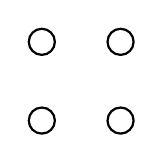
\begin{tikzpicture}[auto,
    specification/.style ={circle, draw, thick}]
   \node[specification] (A) at (0,0)  {};
   \node[specification] (B)  at (0,1)  {};
   \node[specification] (C)  at (1,1)  {};
   \node[specification] (D) at (1,0)  {};
 \end{tikzpicture}\\
 \vspace*{0.1cm}
 A
\end{minipage}\hfill 
  \begin{minipage}{0.24\linewidth}
    \centering
    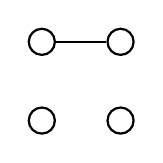
\begin{tikzpicture}[auto,
    specification/.style ={circle, draw, thick}]
   \node[specification] (A) at (0,0)  {};
   \node[specification] (B) at (0,1)  {};
   \node[specification] (C) at (1,1)  {};
   \node[specification] (D) at (1,0)  {};
   \draw[thick] (B) to  (C);
 \end{tikzpicture}\\
 \vspace*{0.1cm}
 B
\end{minipage}\hfill 
  \begin{minipage}{0.24\linewidth}
    \centering
    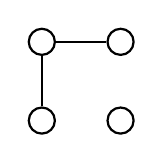
\begin{tikzpicture}[auto,
    specification/.style ={circle, draw, thick}]
   \node[specification] (A) at (0,0)  {};
   \node[specification] (B) at (0,1)  {};
   \node[specification] (C) at (1,1)  {};
   \node[specification] (D) at (1,0)  {};
   \draw[thick] (A) to  (B);
   \draw[thick] (B) to  (C);
 \end{tikzpicture}\\
 \vspace*{0.1cm}
 C
\end{minipage}\hfill 
  \begin{minipage}{0.24\linewidth}
    \centering
    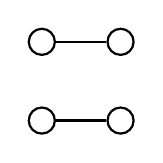
\begin{tikzpicture}[auto,
    specification/.style ={circle, draw, thick}]
   \node[specification] (A)  at (0,0)  {};
   \node[specification] (B)  at (0,1)  {};
   \node[specification] (C)  at (1,1)  {};
   \node[specification] (D) at (1,0)  {};
   \draw[thick] (B) to  (C);
   \draw[thick] (D) to  (A);
 \end{tikzpicture}\\
 \vspace*{0.1cm}
 D
\end{minipage}\hfill

\vspace*{0.5cm}
  \begin{minipage}{0.24\linewidth}
    \centering
    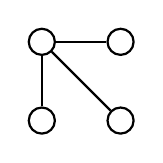
\begin{tikzpicture}[auto,
    specification/.style ={circle, draw, thick}]
   \node[specification] (A) at (0,0)  {};
   \node[specification] (B)  at (0,1)  {};
   \node[specification] (C)  at (1,1)  {};
   \node[specification] (D) at (1,0)  {};
   \draw[thick] (A) to (B);
   \draw[thick] (B) to (C);
      \draw[thick] (B) to (D);
 \end{tikzpicture}\\
 \vspace*{0.1cm}
 E
\end{minipage}\hfill
  \begin{minipage}{0.24\linewidth}
    \centering
    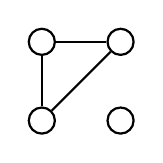
\begin{tikzpicture}[auto,
    specification/.style ={circle, draw, thick}]
   \node[specification] (A) at (0,0)  {};
   \node[specification] (B) at (0,1)  {};
   \node[specification] (C) at (1,1)  {};
   \node[specification] (D) at (1,0)  {};
   \draw[thick] (A) to  (B);
   \draw[thick] (B) to (C);
   \draw[thick] (C) to (A);
 \end{tikzpicture}\\
 \vspace*{0.1cm}
 F
\end{minipage}\hfill
  \begin{minipage}{0.24\linewidth}
    \centering
    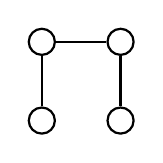
\begin{tikzpicture}[auto,
    specification/.style ={circle, draw, thick}]
   \node[specification] (A) at (0,0)  {};
   \node[specification] (B) at (0,1)  {};
   \node[specification] (C) at (1,1)  {};
   \node[specification] (D) at (1,0)  {};
   \draw[thick] (A) to  (B);
   \draw[thick] (B) to  (C);
      \draw[thick] (C) to (D);
 \end{tikzpicture}\\
 \vspace*{0.1cm}
 G
\end{minipage}\hfill 
  \begin{minipage}{0.24\linewidth}
    \centering
    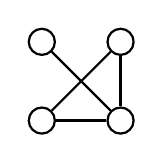
\begin{tikzpicture}[auto,
    specification/.style ={circle, draw, thick}]
   \node[specification] (A)  at (0,0)  {};
   \node[specification] (B)  at (0,1)  {};
   \node[specification] (C)  at (1,1)  {};
   \node[specification] (D) at (1,0)  {};
   \draw[thick] (A) to  (C);
   \draw[thick] (C) to  (D);
   \draw[thick] (D) to (A);
   \draw[thick] (B) to (D);
 \end{tikzpicture}\\
 \vspace*{0.1cm}
 H
\end{minipage}\hfill 

\vspace*{0.5cm}
\flushleft
  \begin{minipage}{0.24\linewidth}
    \centering
    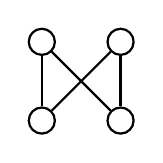
\begin{tikzpicture}[auto,
    specification/.style ={circle, draw, thick}]
   \node[specification] (A) at (0,0)  {};
   \node[specification] (B)  at (0,1)  {};
   \node[specification] (C)  at (1,1)  {};
   \node[specification] (D) at (1,0)  {};
   \draw[thick] (A) to (B);
   \draw[thick] (B) to (D);
   \draw[thick] (D) to (C);
      \draw[thick] (C) to (A);
 \end{tikzpicture}\\
 \vspace*{0.1cm}
 I
\end{minipage}
  \begin{minipage}{0.24\linewidth}
    \centering
    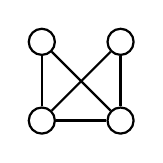
\begin{tikzpicture}[auto,
    specification/.style ={circle, draw, thick}]
   \node[specification] (A) at (0,0)  {};
   \node[specification] (B) at (0,1)  {};
   \node[specification] (C) at (1,1)  {};
   \node[specification] (D) at (1,0)  {};
   \draw[thick] (A) to  (B);
      \draw[thick] (C) to (D);
   \draw[thick] (D) to (A);
   \draw[thick] (A) to (C);
   \draw[thick] (B) to (D);
 \end{tikzpicture}\\
 \vspace*{0.1cm}
 J
\end{minipage} 
  \begin{minipage}{0.24\linewidth}
    \centering
    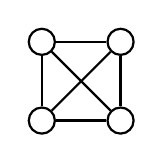
\begin{tikzpicture}[auto,
    specification/.style ={circle, draw, thick}]
   \node[specification] (A) at (0,0)  {};
   \node[specification] (B) at (0,1)  {};
   \node[specification] (C) at (1,1)  {};
   \node[specification] (D) at (1,0)  {};
   \draw[thick] (A) to  (B);
   \draw[thick] (B) to  (C);
      \draw[thick] (C) to (D);
   \draw[thick] (D) to (A);
   \draw[thick] (A) to (C);
   \draw[thick] (B) to (D);
 \end{tikzpicture}\\
 \vspace*{0.1cm}
 K
\end{minipage}  
\end{frame}
\begin{frame}
  \frametitle{1. 树及其性质}
\begin{Thm}
   设树$T$有$p$个顶点,$q$条边,则$q = p-1$。
 \end{Thm}
 \pause
    \centering
    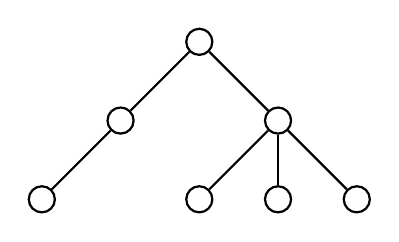
\begin{tikzpicture}[auto,
    specification/.style ={circle, draw, thick}]
   \node[specification] (A)  at (0,0)  {};
   \node[specification] (B)  at (-1,-1)  {};
   \node[specification] (C)  at (1,-1)  {};
   \node[specification] (D)  at (-2,-2)  {};
   \node[specification] (E)  at (0,-2)  {};
   \node[specification] (F)  at (1,-2)  {};
   \node[specification] (G)  at (2,-2)  {};

   \draw[thick] (A) to  (B);
   \draw[thick] (A) to (C);
   \draw[thick] (B) to (D);
   \draw[thick] (C) to (E);
   \draw[thick] (C) to (F);
   \draw[thick] (C) to (G);   
 \end{tikzpicture}
\end{frame}

\begin{frame}
  \frametitle{数学归纳法I}

  \begin{Thm2} 
  $\forall n P(n)$   
\end{Thm2}\pause
\begin{proof}[证明]
  用数学归纳法证明,施归纳于$n$。\pause

  (1)当$n=0$时$P(n)$成立。\pause

  (2)假设当$n=k(k\geq 0)$时$P(n)$成立,往证当$n=k+1$时$P(n)$也成立。
\end{proof}
\pause
(1)$P(0)$\pause

(2)$P(k)\to P(k+1)$

\pause
$P(0)$ \pause $P(1)$ \pause  $P(2)$ \pause $\cdots$
  
\end{frame}

\begin{frame}
\begin{Thm1}
  设树$T$有$p$个顶点,$q$条边,则$q = p-1$。
\end{Thm1}\pause
\begin{proof}[证明]\justifying\let\raggedright\justifying
    \pause用数学归纳法证明,施归纳于顶点数$p$。\pause
    
    (1)当$p=1$时,$q=0$,结论显然成立。\pause

    (2)假设当$p=k$时结论成立,\pause往证当$p=k+1$时结论也成立。\pause设$T$有$k+1$个顶点。\pause $T$中一定存在一个度为1的顶点,\pause这是因为,\pause设$P$为$T$中的一条最长
    路,\pause$v$为$P$的一个端点,\pause则$v$除了$P$上与其关联的边之外,\pause由$T$中无圈知$v$不能再有其他的与$P$上的顶点相关联的边,\pause同时由$P$为一条最长路知$v$不能再有与$P$外
    的顶点相关联的边,\pause因此$v$的度必为1。\pause 去掉$T$中一个度为1的顶点及其与之关联的边,\pause得到的图$T'$连通且无圈,\pause则$T'$是树。\pause $T'$有$k$个顶点,$q-1$条边,\pause由归纳假设,$q-1 = k - 1$, \pause从而$q = (k +1) - 1$, \pause即当$p=k+1$时结论也成立。
\end{proof}
\end{frame}
\begin{frame}
    \begin{Thm1}
  设树$T$有$p$个顶点,$q$条边,则$q = p-1$。
  \end{Thm1}\pause
\centering
  \begin{minipage}{0.24\linewidth}
    \centering
    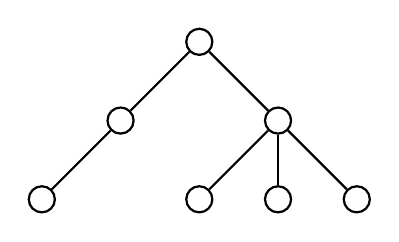
\begin{tikzpicture}[auto,
    specification/.style ={circle, draw, thick}]
   \node[specification] (A)  at (0,0)  {};
   \node[specification] (B)  at (-1,-1)  {};
   \node[specification] (C)  at (1,-1)  {};
   \node[specification] (D)  at (-2,-2)  {};
   \node[specification] (E)  at (0,-2)  {};
   \node[specification] (F)  at (1,-2)  {};
   \node[specification] (G)  at (2,-2)  {};

   \draw[thick] (A) to  (B);
   \draw[thick] (A) to (C);
   \draw[thick] (B) to (D);
   \draw[thick] (C) to (E);
   \draw[thick] (C) to (F);
   \draw[thick] (C) to (G);   
 \end{tikzpicture}
\end{minipage}
\end{frame}
\begin{frame}
  \frametitle{数学归纳法II}

  \begin{Thm2} 
  $\forall n P(n)$   
\end{Thm2}\pause
\begin{proof}[证明]
  用数学归纳法证明,施归纳于$n$。\pause

  (1)当$n=0$时$P(n)$成立。\pause

  (2)假设当$n<k(k\geq 1)$时$P(n)$成立,往证当$n=k$时结论也成立。
\end{proof}
\pause
(1)$P(0)$\pause

(2)$(\forall n< k P(n))\to P(k)$

\pause
$P(0)$ \pause $P(1)$ \pause  $P(2)$ \pause $\cdots$
  
\end{frame}
\begin{frame}
  \begin{Thm1}\small
  设树$T$有$p$个顶点,$q$条边,则$q = p-1$。
\end{Thm1}\pause
  \begin{proof}[证明]\small
      \pause用数学归纳法证明,施归纳于边数$q$。\pause
    
    (1)当$q=0$时,$p=1$,结论显然成立。\pause

    (2)假设当$q<k$时结论成立,\pause往证当$q=k$时结论也成立。\pause 设$T$有$k$条边。\pause去掉
    $T$中的任意一条边,
    \pause得到两个支$T_1$和$T_2$,\pause它们均连通无圈,\pause因此为树。\pause设$T_1$有$p_1$个顶点,
    $k_1$条边,\pause$T_2$有$p_2$个顶点,$k_2$条边,\pause由归纳假设,
    \begin{equation*}
      \begin{split}
        k_1 &= p_1 - 1\\
        k_2 &= p_2 - 1
      \end{split}
    \end{equation*}\pause
    以上两式相加,两边再同时加1,得
    \[k_1 + k_2  + 1 = p_1 + p_2 - 1\]
    \pause从而
    \[k = p - 1 \]
    即当$q=k$时结论也成立。
\end{proof}

\end{frame}
\begin{frame}
\begin{Thm}
  设图$G$有$p$个顶点和$q$条边,如果$G$连通且$q=p-1$,则$G$中无圈。
\end{Thm}
\pause\begin{proof}[证明]
\pause用反证法。\pause假设图$G$中有圈,\pause则去掉圈上的一条边,\pause得到的图仍然为连通的。\pause如果新得到
的图仍然有圈,\pause在圈上再去掉一条边,\pause又会得到一个新的连通的图。\pause如此继续下去,\pause最终会
得到一个连通的没有圈的图。\pause从而最后得到的图中有$p-1$条边,\pause这与去掉
边之前图$G$中的边数$q=p-1$矛盾。 
\end{proof}
  \end{frame}
\begin{frame}
\begin{Thm}
  设图$G$有$p$个顶点和$q$条边,如果$G$无圈且$q=p-1$,则$G$连通。
\end{Thm}
\pause\begin{proof}[证明]
  \pause设图$G$有$k$个支,\pause则图$G$中的每个支连通且没有圈。\pause设第$i$个支中含有$p_i$个顶点,
\pause$q_i$条边,\pause则在第$i$个支中$q_i=p_i-1$。\pause将所有支的边数和顶点数相
加,\pause可得$q = p-k$。\pause于是$k=1$,\pause从而$G$为连通的。
\end{proof}
\end{frame}
\begin{frame}
  \begin{Exercise}\small\justifying\let\raggedright\justifying
  设$a_1$,$a_2$,$\cdots$,$a_p$为$p$个正整数,$p\geq 2$,并且$\sum_{i=1}^pa_i=2(p-1)$。证明:存在一棵具有$p$个顶点的树,它的各个顶点的度分别为$a_1$,$a_2$,$\cdots$,$a_p$。
\end{Exercise}\pause
\begin{proof}[证明]\small\justifying\let\raggedright\justifying
  用数学归纳法证明,施归纳于$p$。\pause

  (1)当$p=2$时,$a_1+a_2=2(2-1)=2$。\pause 由$a_1$,$a_2$为正整数知,$a_1=1$,$a_2=1$。\pause两个顶点之间联结一条边,就构成了一棵满足条件的树。\pause

  (2)假设当$p=k(k\geq 2)$时结论成立,\pause往证当$p=k+1$时结论也成立。\pause设$a_1$,$a_2$,$\cdots$,$a_{k+1}$为$k+1$个正整数,\pause并且$\sum_{i=1}^{k+1}a_i=2(k+1-1)=2k$。\pause此时必存在$s$,$1\leq s \leq k+1$,使得$a_s=1$。\pause否则,如果对任意的$i$,$1\leq i \leq k+1$,\pause有$a_i\geq 2$,\pause那么$\sum_{i=1}^{k+1}a_i\geq 2(k+1)$,\pause与$\sum_{i=1}^{k+1}a_i=2k$矛盾。\pause不妨设$a_{k+1}=1$。\pause此时必存在$t$,$1\leq t \leq k$,$a_t>1$。\pause否则,$a_1=a_2=\cdots=a_k=1$,\pause于是$\sum_{i=1}^{k+1}a_i=k+1<2k$,\pause矛盾。\pause不妨设$a_k>1$。\pause于是$a_1,a_2,\cdots,a_{k-1},a_{k}-1$为正整数,\pause并且$a_1 + a_2 + \cdots + a_{k-1} + (a_{k}-1) = 2(k-1)$。\pause由归纳假设,\pause存在一棵具有$k$个顶点的树,\pause它的各个顶点的度分别为$a_1$,$a_2$,$\cdots$,$a_{k-1}$,$a_k-1$。\pause 在其度为$a_k-1$的顶点上联结一条边和一个顶点,\pause便得到了一棵具有$k+1$个顶点的树,\pause它的各个顶点的度分别为$a_1$,$a_2$,$\cdots$,$a_{k+1}$。
\end{proof}
\end{frame}
\begin{frame}
  \begin{minipage}{0.3\linewidth}
    241131211\pause

    24113111\pause

    2411211\pause

    241111\pause

    23111\pause

    2211\pause

    211\pause

    11\pause
  \end{minipage}
    \begin{minipage}{0.5\linewidth}
    \centering
    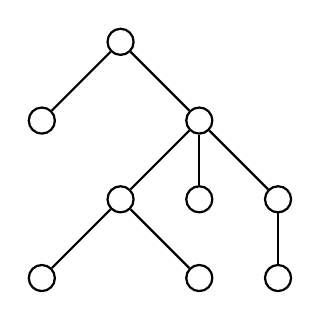
\begin{tikzpicture}[auto,
    specification/.style ={circle, draw, thick}]
   \node[specification] (A)  at (-1,-1)  {};
   \node[specification] (B)  at (0,0)  {};
   \draw[thick] (A) to  (B);\pause
   \node[specification] (C)  at (1,-1)  {};
   \draw[thick] (B) to  (C);\pause
   \node[specification] (D)  at (0,-2)  {};
   \draw[thick] (C) to  (D);\pause
   \node[specification] (E)  at (1,-2)  {};
   \draw[thick] (C) to  (E);\pause
   \node[specification] (F)  at (2,-2)  {};
   \draw[thick] (C) to  (F);\pause
   \node[specification] (G)  at (-1,-3)  {};
   \draw[thick] (D) to  (G);\pause
   \node[specification] (H)  at (1,-3)  {};
   \draw[thick] (D) to  (H);\pause
   \node[specification] (I)  at (2,-3)  {};
   \draw[thick] (F) to  (I);
 \end{tikzpicture}
\end{minipage}

\end{frame}

\section{生成树}


\begin{frame}
  \frametitle{2. 生成树}
  \begin{Def}
    设$G=(V,E)$为一个图,$G$的一个生成子图$T=(V,F)$如果是树,则称$T$为$G$的\alert{生成树}。
  \end{Def}\pause
  \begin{Thm}
    图$G$有生成树的充分必要条件是$G$为一个连通图。
  \end{Thm}
\end{frame}
\section{割点、桥和割集}
\begin{frame}
  \frametitle{3. 割点、桥和割集}
  \begin{Def}
    设$v$为图$G$的一个顶点,如果$G-v$的支数大于$G$的支数,则称顶点$v$为图$G$的一个\alert{割点}。
  \end{Def}
  \centering
    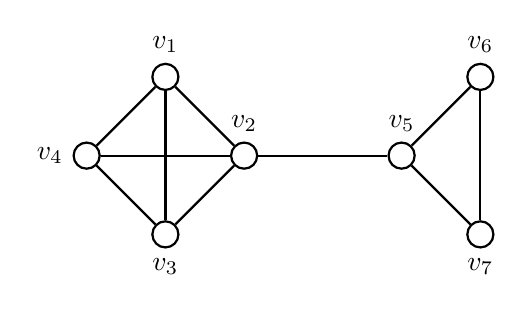
\begin{tikzpicture}[auto,
    specification/.style ={circle, draw, thick}]
   \node[specification] (A) [label=90:$v_1$] at (1,1)  {};
   \node[specification] (B) [label=90:$v_2$] at (2,0)  {};
   \node[specification] (C) [label=-90:$v_3$] at (1,-1)  {};
   \node[specification] (D) [label=180:$v_4$] at (0,0)  {};
   \node[specification] (E) [label=90:$v_5$] at (4,0) {};
   \node[specification] (F) [label=90:$v_6$] at (5,1) {};
   \node[specification] (G) [label=-90:$v_7$] at (5,-1) {};
   \draw[thick] (A) to  (B);
   \draw[thick] (B) to  (C);
   \draw[thick] (C) to  (D);
   \draw[thick] (D) to  (A);
   \draw[thick] (A) to  (C);
   \draw[thick] (B) to  (D);   
   \draw[thick] (B) to  (E);
   \draw[thick] (E) to  (F);
   \draw[thick] (F) to  (G);
   \draw[thick] (G) to  (E);
 \end{tikzpicture}  

\end{frame}

\begin{frame}
  \frametitle{3. 割点、桥和割集}
  \begin{Thm}
    设$v$为连通图$G=(V,E)$的一个割点,则下列命题等价:
    \begin{enumerate}[(1)]
    \item $v$为图$G$的一个割点;
    \item \justifying\let\raggedright\justifying
集合$V\setminus \{v\}$有一个二划分$\{U,W\}$, 使得对任意的$u \in U$,$w \in W$,$v$在联结$u$和$w$的每条路上;
    \item 存在与$v$不同的两个顶点$u$和$w$,使得$v$在每一条$u$与$w$间的路上。
    \end{enumerate}
  \end{Thm}
  \centering
    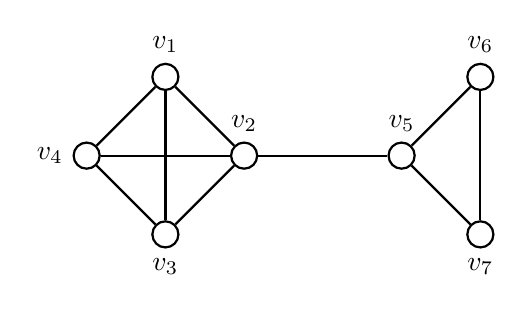
\begin{tikzpicture}[auto,
    specification/.style ={circle, draw, thick}]
   \node[specification] (A) [label=90:$v_1$] at (1,1)  {};
   \node[specification] (B) [label=90:$v_2$] at (2,0)  {};
   \node[specification] (C) [label=-90:$v_3$] at (1,-1)  {};
   \node[specification] (D) [label=180:$v_4$] at (0,0)  {};
   \node[specification] (E) [label=90:$v_5$] at (4,0) {};
   \node[specification] (F) [label=90:$v_6$] at (5,1) {};
   \node[specification] (G) [label=-90:$v_7$] at (5,-1) {};
   \draw[thick] (A) to  (B);
   \draw[thick] (B) to  (C);
   \draw[thick] (C) to  (D);
   \draw[thick] (D) to  (A);
   \draw[thick] (A) to  (C);
   \draw[thick] (B) to  (D);   
   \draw[thick] (B) to  (E);
   \draw[thick] (E) to  (F);
   \draw[thick] (F) to  (G);
   \draw[thick] (G) to  (E);
 \end{tikzpicture}  

\end{frame}

\begin{frame}
  \frametitle{3. 割点、桥和割集}
  \begin{Def}
   图$G$的一条边$x$称为$G$的一座\alert{桥},如果$G-x$的支数大于$G$的支数。
  \end{Def}
  \centering
    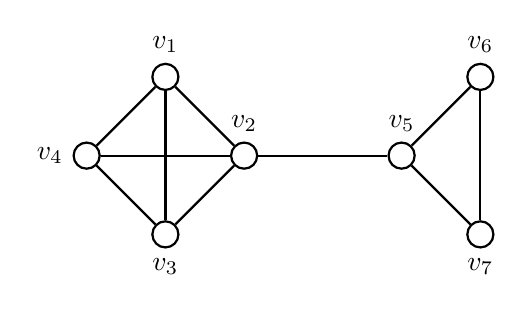
\begin{tikzpicture}[auto,
    specification/.style ={circle, draw, thick}]
   \node[specification] (A) [label=90:$v_1$] at (1,1)  {};
   \node[specification] (B) [label=90:$v_2$] at (2,0)  {};
   \node[specification] (C) [label=-90:$v_3$] at (1,-1)  {};
   \node[specification] (D) [label=180:$v_4$] at (0,0)  {};
   \node[specification] (E) [label=90:$v_5$] at (4,0) {};
   \node[specification] (F) [label=90:$v_6$] at (5,1) {};
   \node[specification] (G) [label=-90:$v_7$] at (5,-1) {};
   \draw[thick] (A) to  (B);
   \draw[thick] (B) to  (C);
   \draw[thick] (C) to  (D);
   \draw[thick] (D) to  (A);
   \draw[thick] (A) to  (C);
   \draw[thick] (B) to  (D);   
   \draw[thick] (B) to  (E);
   \draw[thick] (E) to  (F);
   \draw[thick] (F) to  (G);
   \draw[thick] (G) to  (E);
 \end{tikzpicture}  

\end{frame}

\begin{frame}
  \frametitle{3. 割点、桥和割集}
  \begin{Thm}
    设$x$为连通图$G=(V,E)$的一条边,则下列命题等价:
    \begin{enumerate}[(1)]
    \item $x$为$G$的桥;
    \item $x$不在$G$的任一圈上;
    \item 存在$V$的一个划分$\{U,W\}$,使得对任意的$u \in U, w \in W$,$x$在每一条联结$u$与$w$的路上;
    \item 存在$G$的不同顶点$u$和$v$,使得边$x$在联结$u$和$v$的每条路上。
    \end{enumerate}
  \end{Thm}
  \centering
    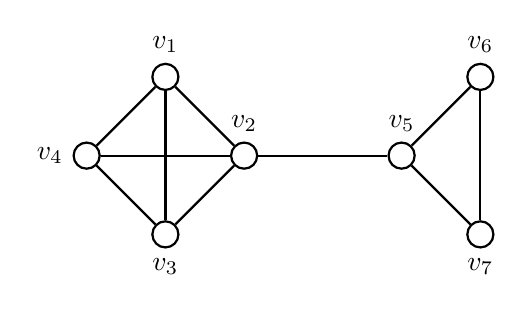
\begin{tikzpicture}[auto,
    specification/.style ={circle, draw, thick}]
   \node[specification] (A) [label=90:$v_1$] at (1,1)  {};
   \node[specification] (B) [label=90:$v_2$] at (2,0)  {};
   \node[specification] (C) [label=-90:$v_3$] at (1,-1)  {};
   \node[specification] (D) [label=180:$v_4$] at (0,0)  {};
   \node[specification] (E) [label=90:$v_5$] at (4,0) {};
   \node[specification] (F) [label=90:$v_6$] at (5,1) {};
   \node[specification] (G) [label=-90:$v_7$] at (5,-1) {};
   \draw[thick] (A) to  (B);
   \draw[thick] (B) to  (C);
   \draw[thick] (C) to  (D);
   \draw[thick] (D) to  (A);
   \draw[thick] (A) to  (C);
   \draw[thick] (B) to  (D);   
   \draw[thick] (B) to  (E);
   \draw[thick] (E) to  (F);
   \draw[thick] (F) to  (G);
   \draw[thick] (G) to  (E);
 \end{tikzpicture}  

\end{frame}

\begin{frame}
  \frametitle{3. 割点、桥和割集}
  \begin{Def}
    设$G = (V,E)$为图,$S \subseteq E$。如果从$G$中去掉$S$中的所有边得到的图$G-S$的支数大于$G$的支数,而去掉$S$的任一真子集中的边得到的图的支数不大于$G$的支数,则称$S$为$G$的一个\alert{割集}。
  \end{Def}
  \centering
    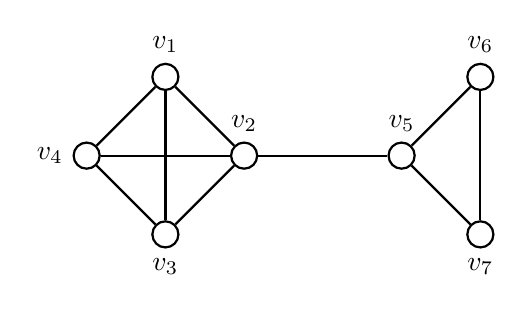
\begin{tikzpicture}[auto,
    specification/.style ={circle, draw, thick}]
   \node[specification] (A) [label=90:$v_1$] at (1,1)  {};
   \node[specification] (B) [label=90:$v_2$] at (2,0)  {};
   \node[specification] (C) [label=-90:$v_3$] at (1,-1)  {};
   \node[specification] (D) [label=180:$v_4$] at (0,0)  {};
   \node[specification] (E) [label=90:$v_5$] at (4,0) {};
   \node[specification] (F) [label=90:$v_6$] at (5,1) {};
   \node[specification] (G) [label=-90:$v_7$] at (5,-1) {};
   \draw[thick] (A) to  (B);
   \draw[thick] (B) to  (C);
   \draw[thick] (C) to  (D);
   \draw[thick] (D) to  (A);
   \draw[thick] (A) to  (C);
   \draw[thick] (B) to  (D);   
   \draw[thick] (B) to  (E);
   \draw[thick] (E) to  (F);
   \draw[thick] (F) to  (G);
   \draw[thick] (G) to  (E);
 \end{tikzpicture}  

\end{frame}

\begin{frame}  
  \frametitle{习题}

  \begin{Exercise}
  分别画出具有4、5、6、7个顶点的所有树(同构的只算一个)。
  \end{Exercise}
  % \begin{Exercise}
  % 令$G$为一个有$p$个顶点,$k$个支的森林。证明:$G$有$p-k$条边。
  % \end{Exercise}
  % \begin{Exercise}
  %   设$a_1$,$a_2$,$\cdots$,$a_p$为$p$个正整数,$p \geq 2$,并且
  %   $\sum_{i=1}^pa_i=2(p-1)$。证明:存在一个具有$p$个顶点的树,它的各个顶点的度
  %   分别为$a_1$,$a_2$,$\cdots$,$a_p$。
  % \end{Exercise}
\end{frame}

\end{CJK*}
\end{document}

%%% Local Variables:
%%% mode: latex
%%% TeX-master: t
%%% End:
